%% Poster Científico — Invernadero Andino
%% Basado en template de latex-document-skill (ndpvt-web)
%% tikzposter | Portrait A0 | 2-column | Olive scheme
%% Compilar: pdflatex poster_cientifico.tex

\documentclass[25pt, portrait, margin=15mm,
    innermargin=15mm, blockverticalspace=12mm, colspace=20mm]{tikzposter}

\usepackage[utf8]{inputenc}
\usepackage[LY1]{fontenc}
\usepackage{amsmath,amssymb}
\usepackage{graphicx}
\usepackage{booktabs}
\usepackage{enumitem}
\usepackage{pgfplots}
\pgfplotsset{compat=1.18}
\usepackage{qrcode}
\usepackage{newpxtext}
\geometry{paperwidth=841mm, paperheight=1189mm}

\renewcommand{\familydefault}{\rmdefault}

%% ── PALETA OLIVE ──
\definecolor{olive}{HTML}{4a5d23}
\definecolor{olivelight}{HTML}{6b8e23}
\definecolor{olivebg}{HTML}{f0f5e8}
\definecolor{gold}{HTML}{c8a84e}
\definecolor{goldbg}{HTML}{f5f0e8}
\definecolor{darktext}{HTML}{1f2937}
\definecolor{lightbg}{HTML}{faf8f4}

%% ── TITLE STYLE ──
\definetitlestyle{OliveTitle}{
    width=\paperwidth, roundedcorners=0, linewidth=0pt, innersep=2cm,
    titletotopverticalspace=0mm, titletoblockverticalspace=20mm
}{
    \begin{scope}[line width=\titlelinewidth, rounded corners=\titleroundedcorners]
        \fill[color=olive] (\titleposleft,\titleposbottom) rectangle (\titleposright,\titlepostop);
        \fill[color=gold] (\titleposleft,\titleposbottom) rectangle (\titleposright,\titleposbottom+0.5cm);
    \end{scope}
}

%% ── BLOCK STYLE ──
\defineblockstyle{OliveBlock}{
    titlewidthscale=1, bodywidthscale=1, titleleft,
    titleoffsetx=0pt, titleoffsety=0pt, bodyoffsetx=0pt, bodyoffsety=0pt,
    bodyverticalshift=0pt, roundedcorners=8, linewidth=2pt,
    titleinnersep=10mm, bodyinnersep=15mm
}{
    \draw[color=olivelight!40, fill=white, rounded corners=\blockroundedcorners, line width=1pt]
        (blockbody.south west) rectangle (blockbody.north east);
    \ifBlockHasTitle
        \draw[color=olive, fill=olive, rounded corners=\blockroundedcorners]
            (blocktitle.south west) rectangle (blocktitle.north east);
    \fi
}

\usetheme{Default}
\usetitlestyle{OliveTitle}
\useblockstyle{OliveBlock}

\colorlet{backgroundcolor}{white}
\colorlet{framecolor}{olivelight}
\colorlet{titlebgcolor}{olive}
\colorlet{titlefgcolor}{white}
\colorlet{blocktitlebgcolor}{olive}
\colorlet{blocktitlefgcolor}{white}
\colorlet{blockbodybgcolor}{white}
\colorlet{blockbodyfgcolor}{darktext}

\tikzposterlatexaffectionproofoff

%% ── TITLE ──
\title{\parbox{0.90\linewidth}{\centering\textbf{%
    Sistema de optimización de clima en invernaderos andinos\\[0.2em]
    mediante modelos acoplados de cuatro variables y control predictivo con TinyML embebido}}}
\author{Lenin Yudain Coronel Pacheco}
\institute{Ingenieria de Sistemas, Universidad Distrital Francisco Jose de Caldas, Bogotá D.C., Colombia\\[0.3em]
           \texttt{lycoronelp@udistrital.edu.co}}

\begin{document}

\maketitle

\begin{columns}

%% ══════════════════════════════════════════════════════════════
%% COL 1
%% ══════════════════════════════════════════════════════════════
\column{0.50}

\block{1. Introducción}{
    La agricultura altoandina colombiana (2640 msnm, $\sim$750 hPa) enfrenta tres brechas que este proyecto aborda de forma integrada:

    \vspace{1em}
    \begin{itemize}[leftmargin=*, itemsep=0.8em]
        \item \textbf{Falta de automatización:} control manual, consumo de agua 40--60\% superior al óptimo [1]
        \item \textbf{Modelos no calibrados} para altitud andina: $\gamma$ varia 28\% vs nivel del mar [3]
        \item \textbf{Brecha en computación embebida:} sin integración documentada de EDOs + TinyML + MPC en un MCU [2,6]
    \end{itemize}

    \vspace{1em}
    \coloredbox[bgcolor=olivebg, fgcolor=darktext, roundedcorners=5]{%
        \textbf{Pregunta:} $i$Es posible implementar MPC con EDOs acopladas ($T$, $W$, $C$, $E_t$) y TinyML en un ESP32-S3 que reduzca agua $\ge$ 40\% y mejore rendimiento $\ge$ 5\% en invernaderos altoandinos, sin conectividad externa?
    }
}

\block{2. Objetivos espec{\'\i}ficos}{
    \begin{itemize}[leftmargin=*, itemsep=0.7em]
        \item[\textbf{OE1}] \textbf{Modelo calibrado} (M1--4): EDOs con corrección psicométrica, sensibilidad global (Morris, Sobol) e incertidumbre (Monte Carlo $N=10^4$ [14]). RMSE $<1\,^{\circ}$C, $<5\%$ HR, $<50$ ppm CO$_2$
        \item[\textbf{OE2}] \textbf{RL-Guided MPC} (M3--7): $H_p$ 5--15 min en ESP32-S3. Seguimiento HR $\le\pm5\%$, ejecución $<50$ ms
        \item[\textbf{OE3}] \textbf{Módulo TinyML} (M5--8): red superficial ($<5$K params, $<50$ KB INT8). Predice radiación solar y $T_{\text{ext}}$. Latencia $<100$ ms, $<50$ mW
        \item[\textbf{OE4}] \textbf{Validación integral} (M8--12): diseño ABA 12 semanas [15] en piloto 200 m$^2$ con lechuga. Agua $\ge$ 40\%, rendimiento $\ge$ 5\% ($p<0.05$)
    \end{itemize}
}

\block{3. Modelo matemático}{
    Cuatro EDOs acoplan la dinámica del microclima interior:\\[0.5em]

    \textbf{Balance energético (EDO-1)}
    \[ C_p\frac{dT_{\text{in}}}{dt} = \frac{Q_{\text{rad}}+Q_{\text{calef}}-Q_{\text{vent}}-Q_{\text{transp}}}{V} \]

    \textbf{Balance de humedad (EDO-2)}
    \[ \frac{dW_{\text{in}}}{dt} = \frac{W_{\text{out}}\dot V + E_{\text{tr}} - W_{\text{in}}\dot V}{V} \]

    \textbf{Balance de CO$_2$ (EDO-3)}
    \[ \frac{dC_{\text{in}}}{dt} = \frac{C_{\text{out}}\dot V - P_n A_{\text{leaf}} + R_d A_{\text{leaf}} - C_{\text{in}}\dot V}{V} \]

    \textbf{Penman-Monteith (EDO-4)}
    \[ \text{ET}_0 = \frac{\Delta(R_n-G)+\rho c_p(e_s-e_a)/r_a}{\Delta+\gamma(1+r_s/r_a)} \]

    \textbf{Corrección psicométrica por altitud}
    \[ \gamma = \frac{c_p\cdot P}{0.622\cdot L_v} \qquad
       \gamma_{\text{Bogotá}} = \frac{1003\cdot 750}{0.622\cdot 2.501\cdot 10^6} \approx 0.048\;\text{kPa}/^{\circ}\text{C} \]
    \begin{center}\small 28\% menor que $\gamma_{\text{SL}}\approx 0.0665$ \textrightarrow\ error sin corrección [9]\end{center}
}

\block{4. Módulo TinyML y control}{
    \textbf{TinyML} --- Red superficial (150--300 params [13]) cuantizada INT8 via TFLite Micro, $<50$ KB. Predice radiación solar (RMSE $<50$ W/m$^2$) y $T_{\text{ext}}$ (RMSE $<1\,^{\circ}$C).

    Ningun trabajo previo integra TinyML con resolución de EDOs en un MCU [2,6].

    \textbf{RL-Guided MPC} --- RL construye el costo terminal [12]:
    \[ J^{\text{RL}}_{\text{MPC}} = \sum_{k=0}^{H_p} \|x_k-x_{\text{ref},k}\|_Q^2 + V^{\text{RL}}(x_{H_p}) \]

    MPC ofrece estabilidad nominal (HR $\le\pm5\%$); RL maneja incertidumbre en perturbaciones climaticas [11]. Primera implementación de esta arquitectura hibrida en un microcontrolador.
}

%% ══════════════════════════════════════════════════════════════
%% COL 2
%% ══════════════════════════════════════════════════════════════
\column{0.50}

\block{5. Arquitectura del sistema}{
    \begin{tikzfigure}[Arquitectura ciber-físico implementada]
        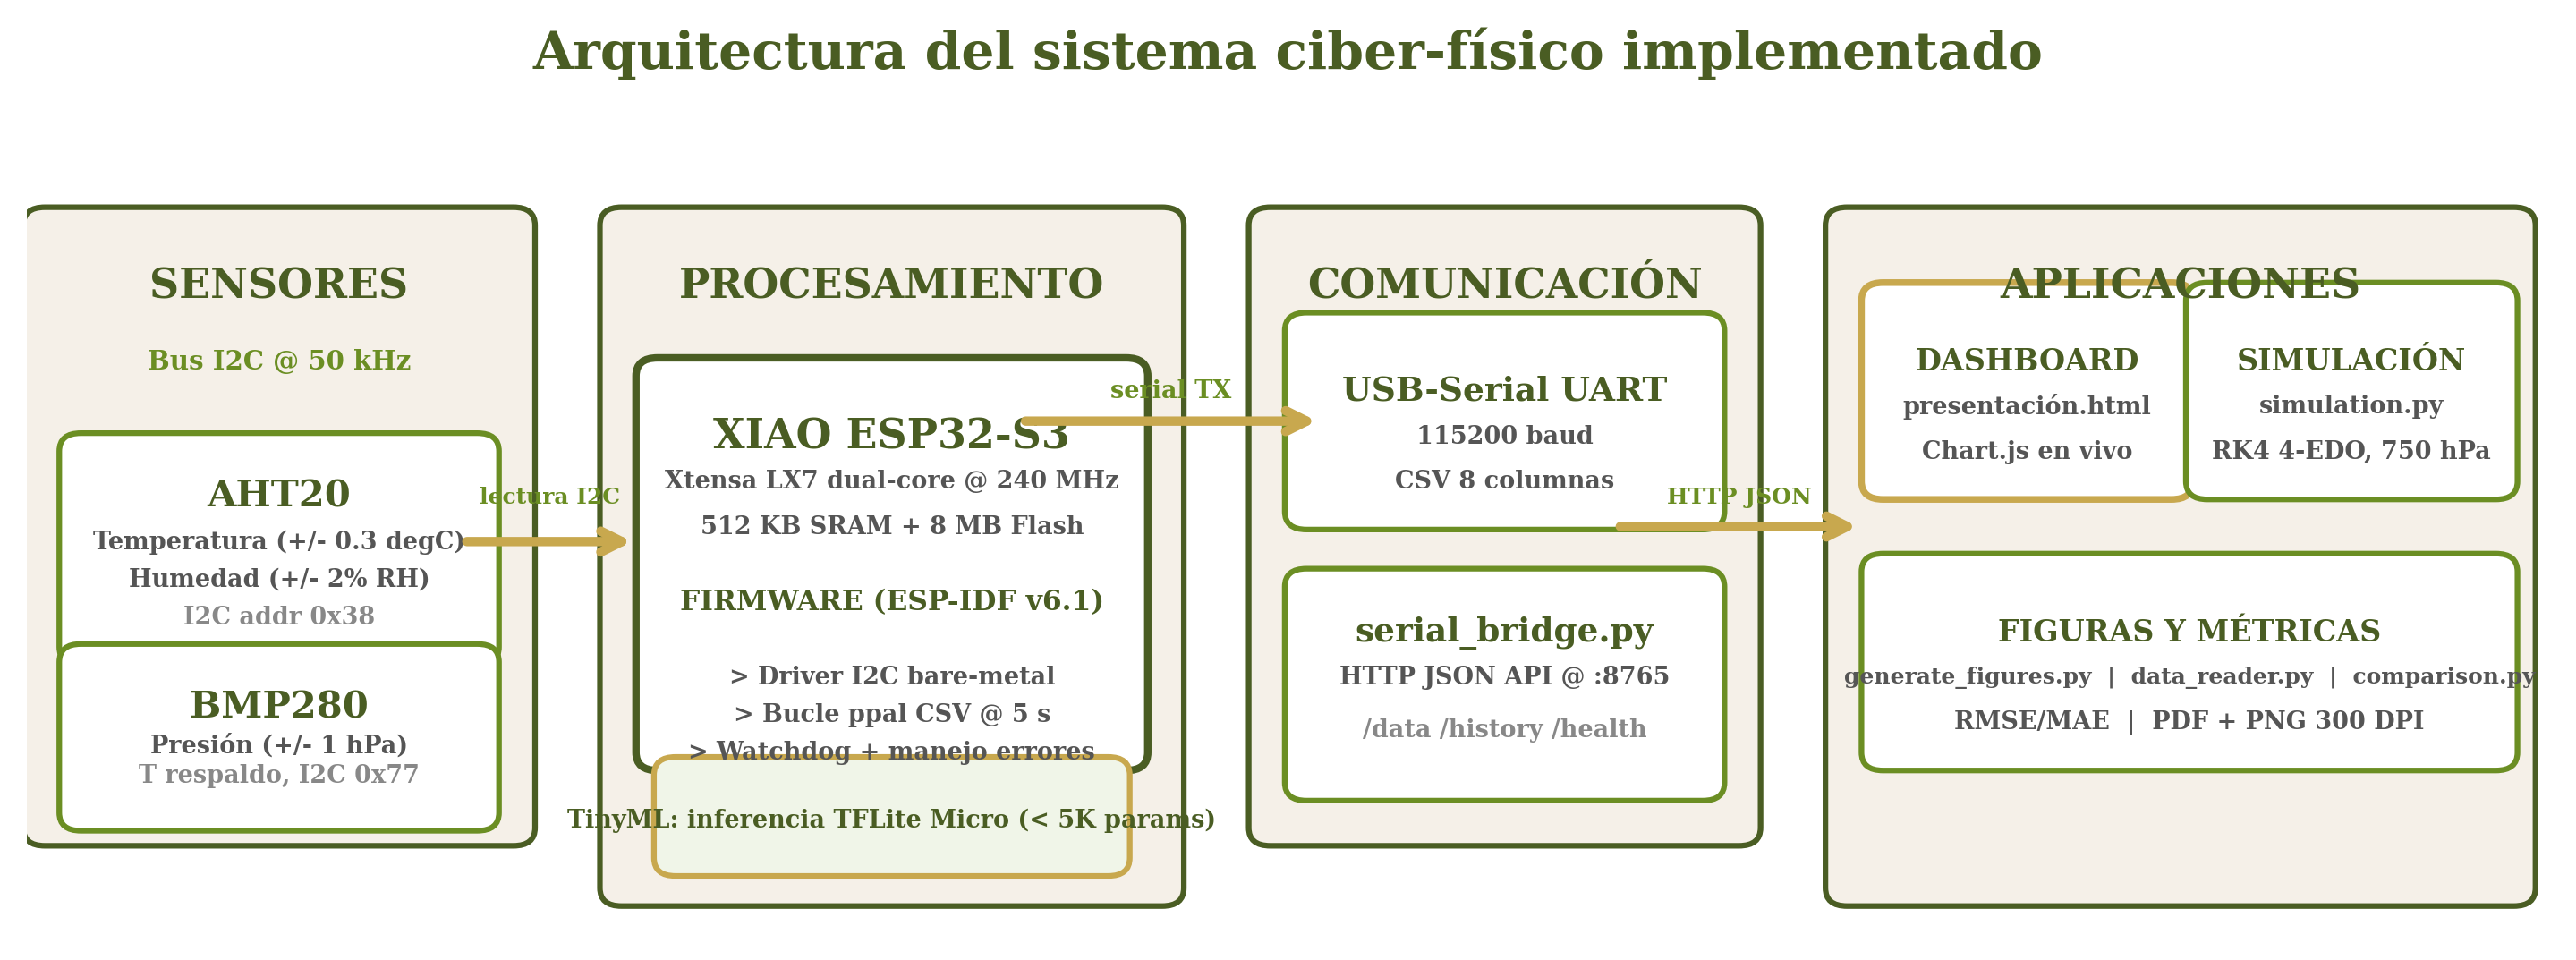
\includegraphics[width=0.95\linewidth]{figures/fig3_arch.png}
    \end{tikzfigure}

    Flujo: sensores AHT20+BMP280 (I$^2$C) $\rightarrow$ ESP32-S3 (firmware C) $\rightarrow$ serial USB-CSV $\rightarrow$ bridge Python HTTP $\rightarrow$ dashboard, simulación RK4, generación de poster.

    \vspace{1em}
    {\large
    \begin{tabular}{ll}
        \textbf{MCU} & XIAO ESP32S3 (240 MHz LX7 dual-core, 512 KB SRAM + 8 MB PSRAM) \\
        \textbf{Sensores} & AHT20 ($\pm0.3\,^{\circ}$C, $\pm2\%$ RH) + BMP280 ($\pm1$ hPa) \\
        \textbf{Bus / FW} & I$^2$C1 @ 50 kHz \hfill Bare-metal C, ESP-IDF v6.1 \\
        \textbf{Salida} & CSV 8 col @ 115200 baud, 5 s \hfill Python HTTP JSON @ :8765 \\
    \end{tabular}
    }
}

\block{6. Resultados experimentales}{
    \begin{tikzfigure}[Temperatura y humedad relativa]
        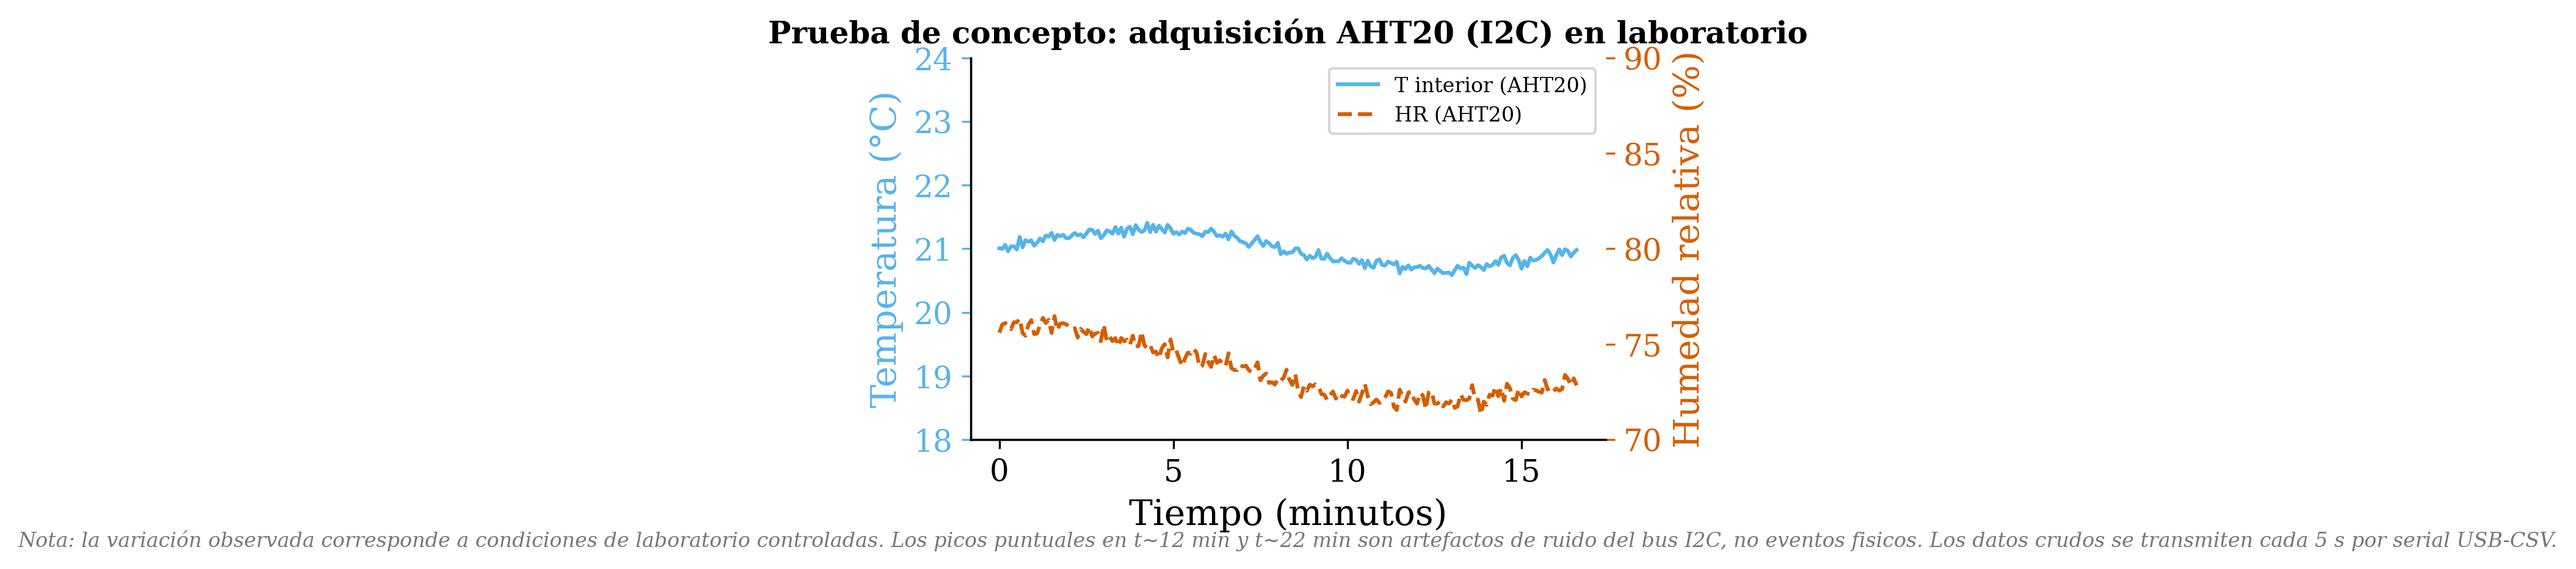
\includegraphics[width=0.95\linewidth]{figures/fig1_temp_hum.png}
    \end{tikzfigure}
    \begin{tikzfigure}[Presión y CO$_2$]
        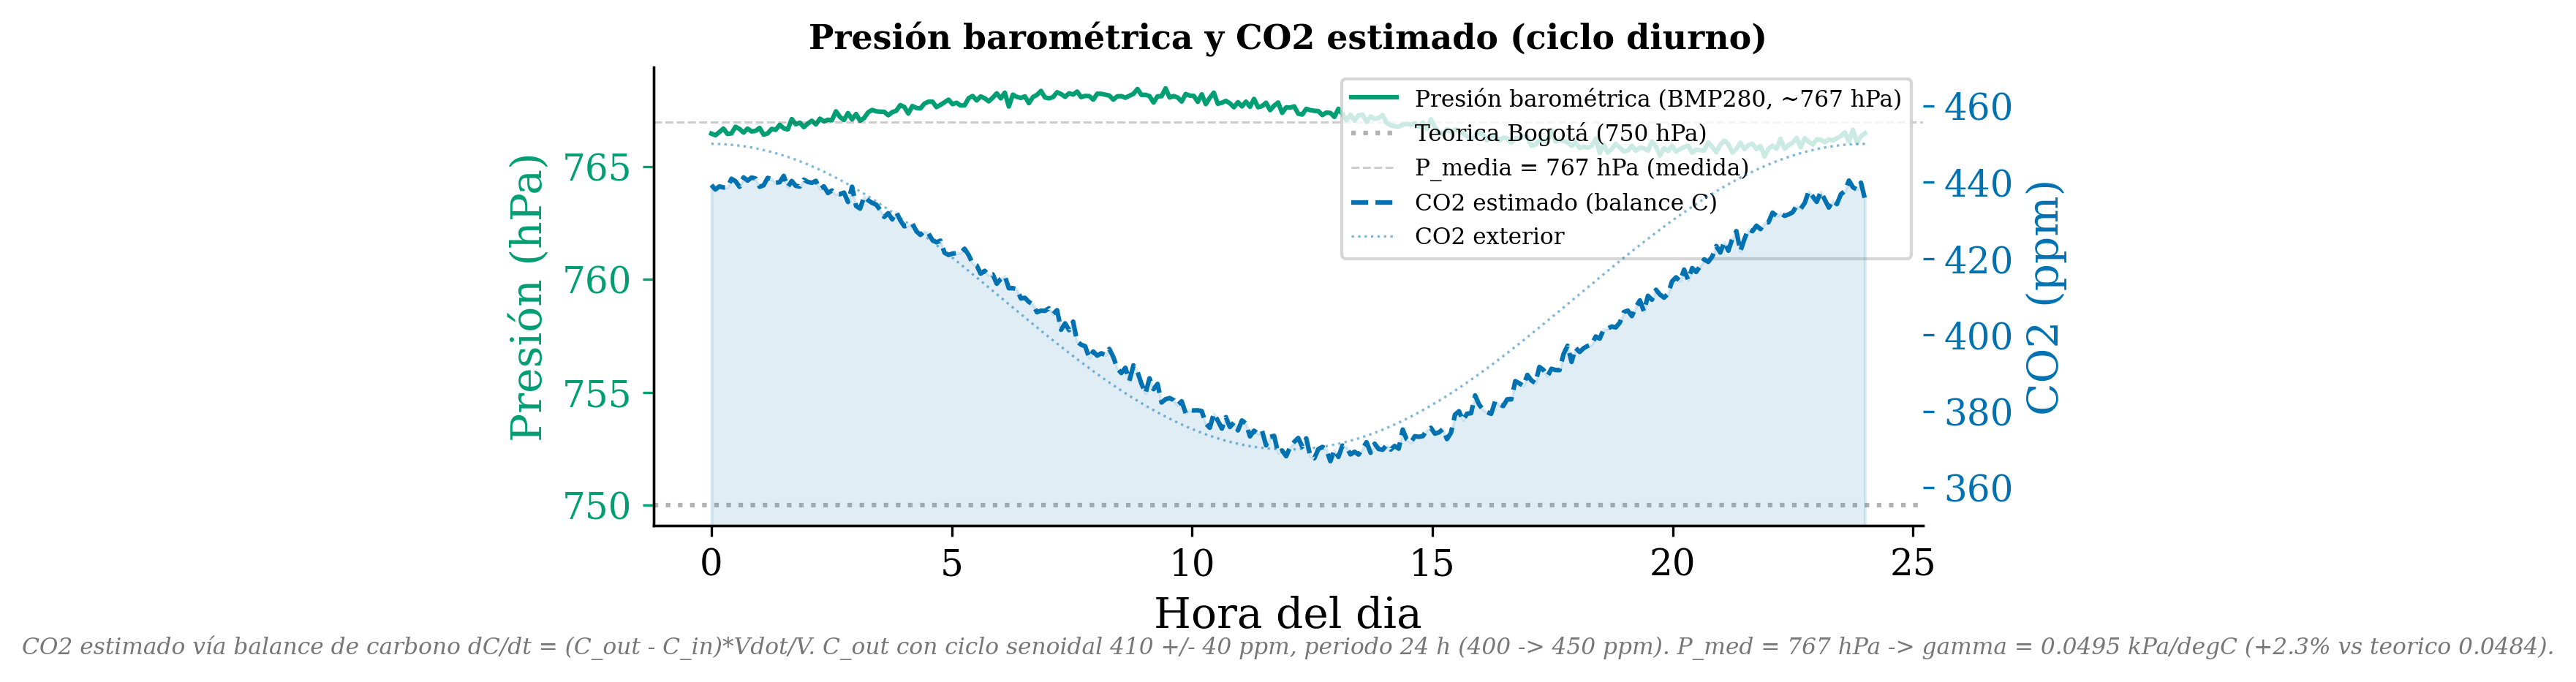
\includegraphics[width=0.95\linewidth]{figures/fig2_press_co2.png}
    \end{tikzfigure}

    \textbf{Fig. 2:} $T_{\text{in}}$ (azul) y HR (naranja) vía AHT20 durante $\sim$11 min @ 5 s. Exactitud $\pm0.3\,^{\circ}$C, $\pm2\%$ RH.

    \textbf{Fig. 3:} Presión barométrica (BMP280, verde) con referencia 750 hPa (punteada) y CO$_2$ estimado (morado). Presión $\sim$767 hPa (2.3\% sobre teórica).
}

\block{7. Simulación numérica RK4}{
    \begin{tikzfigure}[Simulación RK4 de 7 dias -- Bogotá 2640 msnm]
        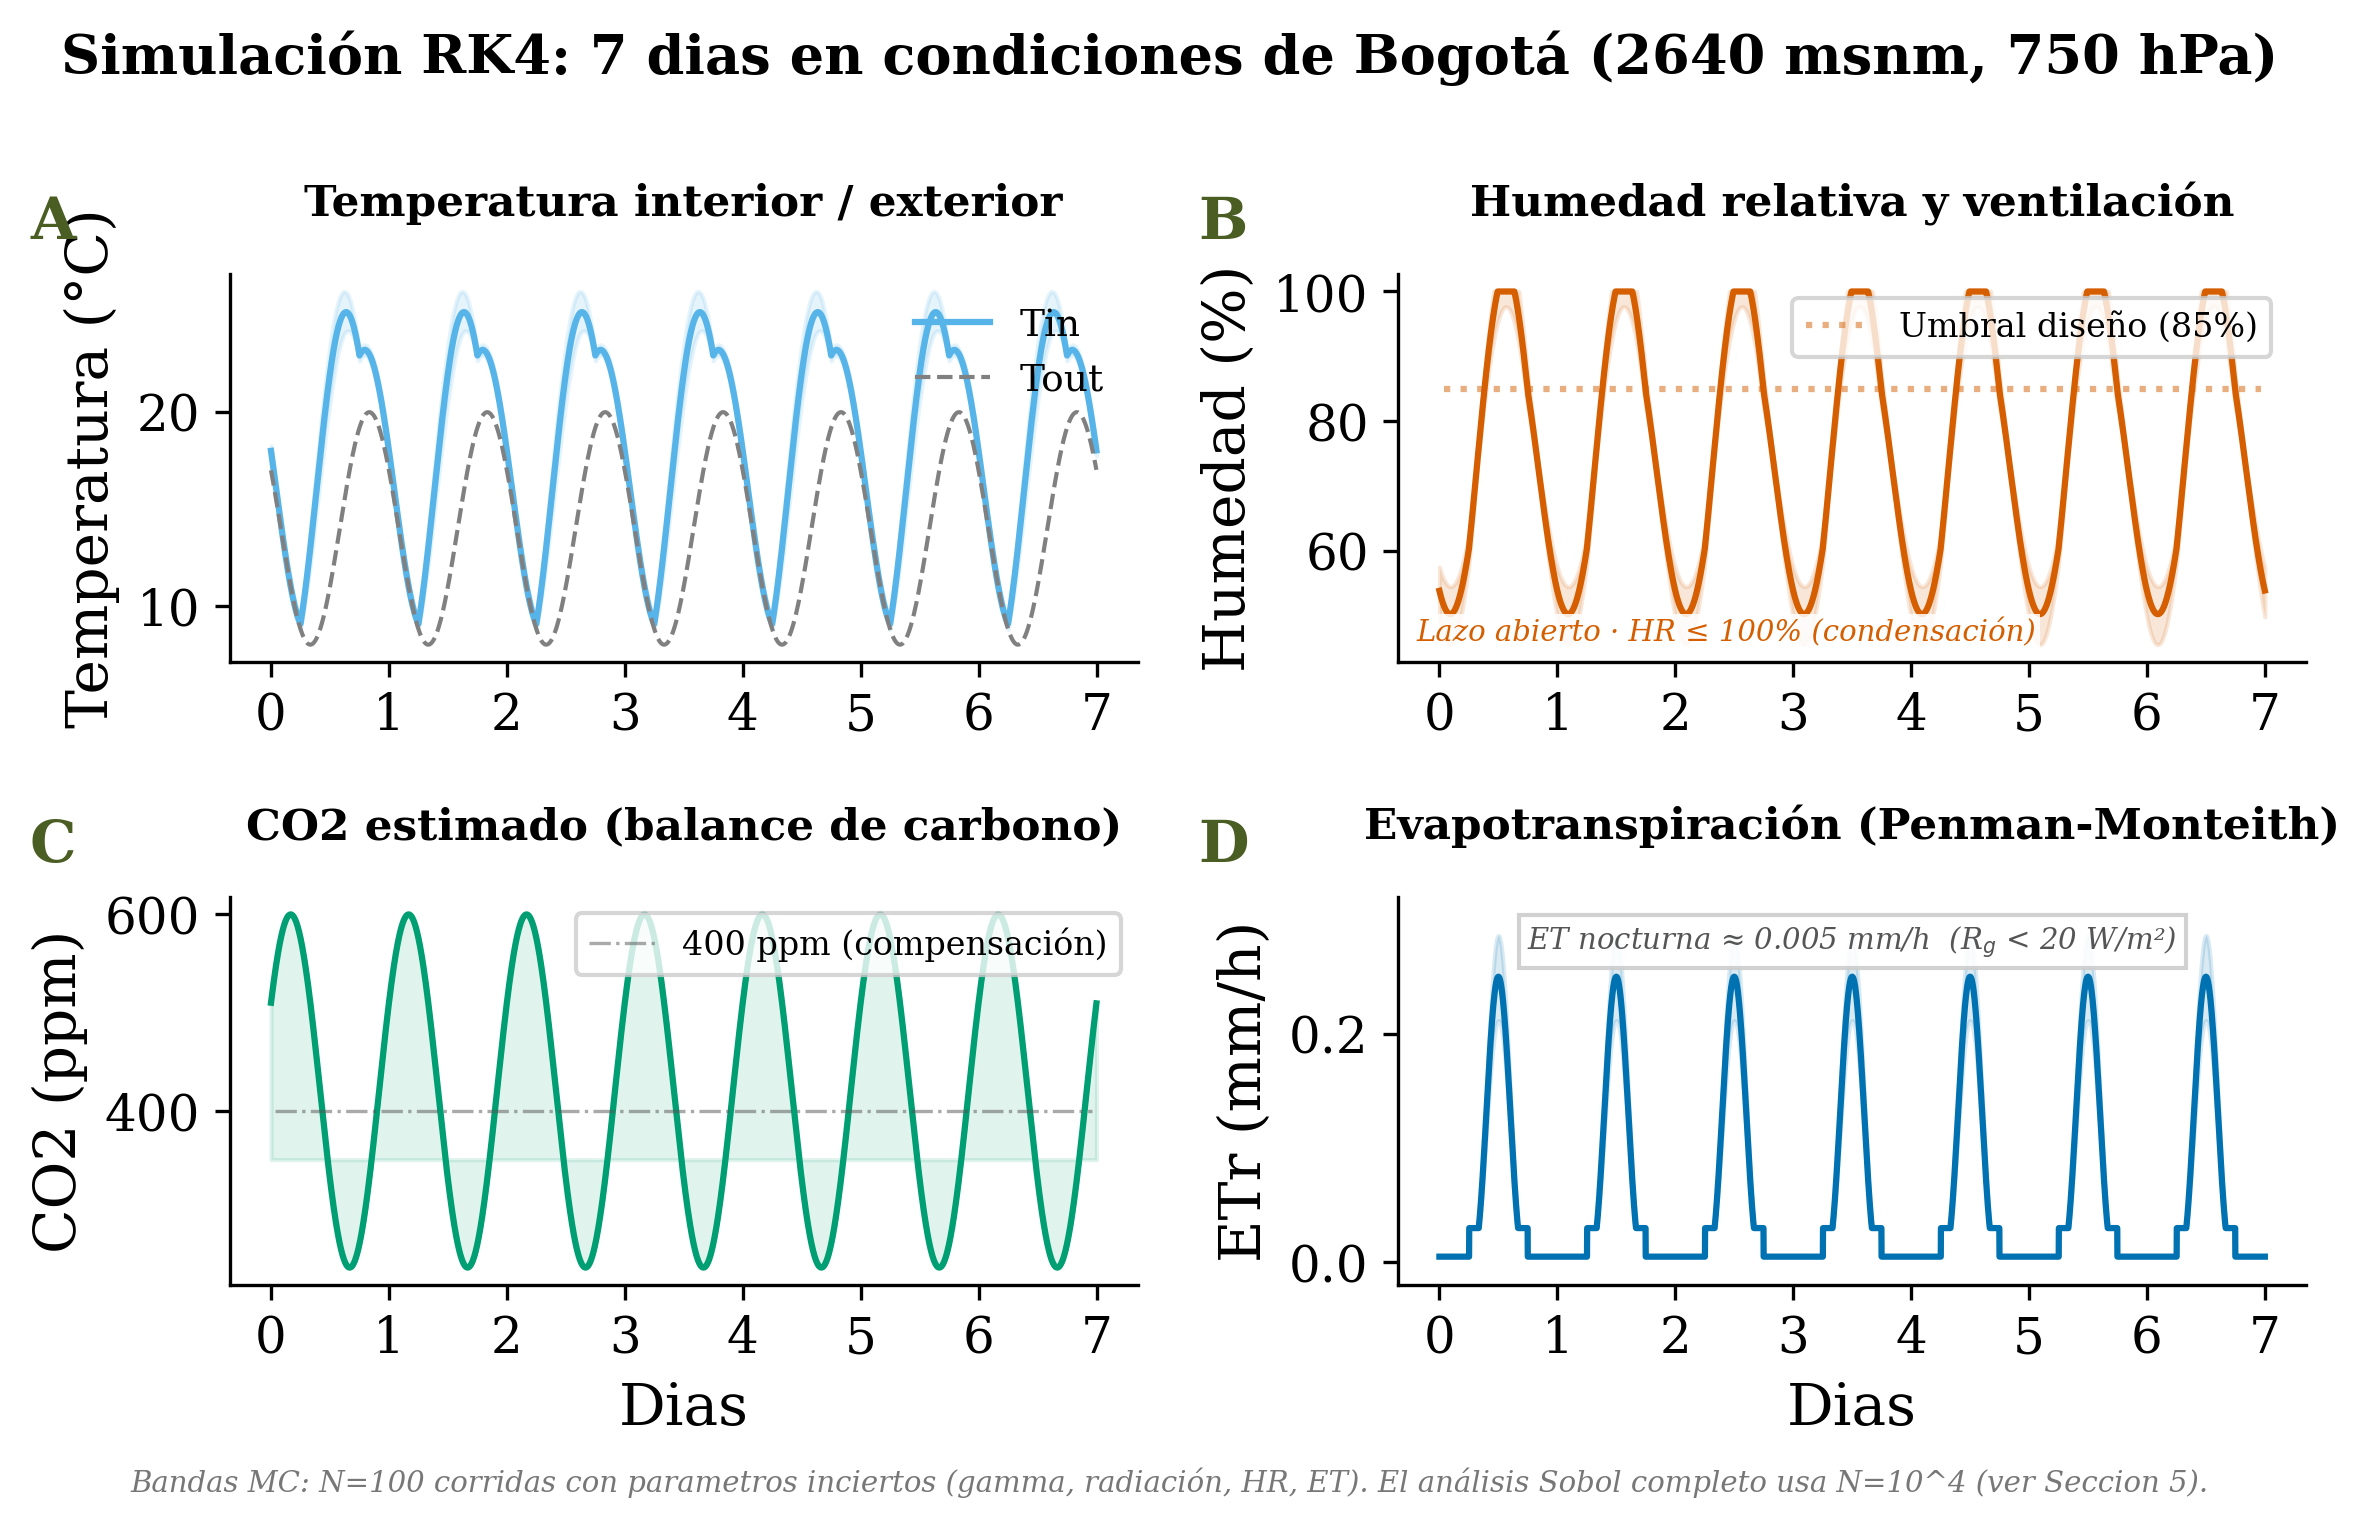
\includegraphics[width=0.95\linewidth]{figures/fig4_sim.png}
    \end{tikzfigure}

    \textbf{Fig. 4:} RK4 con $P=750$ hPa, $\gamma=0.048$ kPa/$^{\circ}$C. Paneles: (A) $T$ in vs ext; (B) HR con ventilación al 85\%; (C) CO$_2$ interior; (D) Et$_0$ corregida por altitud.
}

\block{8. Brechas y métricas}{
    {\large
    \begin{tabular}{p{0.38\linewidth}p{0.55\linewidth}}
        \toprule
        \textbf{Vacio en la literatura} & \textbf{Abordado mediante} \\
        \midrule
        Modelos no calibrados para clima andino & Corrección psicométrica + validación a 2640 msnm \\
        Sin análisis de incertidumbre & Sobol + Monte Carlo con $N=10^4$ \\
        Acoplamiento incompleto de variables & 4 EDOs acopladas ($T$, $W$, $C$, $E_t$) \\
        RL-Guided MPC no implementado en HW & Portabilidad a ESP32-S3 con horizonte reducido \\
        TinyML sin integración con simulación & Pipeline RK4 + inferencia TFLite Micro \\
        \bottomrule
    \end{tabular}
    }

    \vspace{1em}
    \begin{center}
    {\large
    \begin{tabular}{cccccc}
        \textbf{RMSE $T_{\text{in}}$} & \textbf{RMSE $W_{\text{in}}$} & \textbf{RMSE CO$_2$} & \textbf{Ahorro agua} & \textbf{Mejora rend.} & \textbf{Costo sist.} \\
        $<1\,^{\circ}$C & $<5\%$ HR & $<50$ ppm & $\ge40\%$ & $\ge5\%$ & $<\$2{,}500$
    \end{tabular}
    }
    \end{center}
}

\block{Referencias \& Contacto}{
    {\footnotesize
    [1] Zhang et al. (2022). \textit{Water}, 14(23), 3941. \hfill
    [2] Banakar \& Goudar (2022). \textit{Internet of Things}, 19, 100548. \hfill
    [3] Lopez-Cruz et al. (2018). \textit{Eur. J. Hort. Sci.}, 83(5), 269. \hfill
    [4] Queralt (2024). PhD Thesis, Univ. de Liege. \hfill
    [5] Chen et al. (2021). \textit{Biosyst. Eng.}, 204, 1. \hfill
    [6] Morales-Garcia et al. (2023). \textit{J. Supercomput.}, 79, 10277. \hfill
    [7] Ihoume et al. (2022). \textit{Smart Agric. Tech.}, 2, 100039. \hfill
    [8] Stanghellini (1987). PhD Thesis, Wageningen. \hfill
    [9] Islam et al. (2012). \textit{Trans. ASABE}, 55(6), 2135. \hfill
    [10] van Straten et al. (2020). CRC Press. \hfill
    [11] Hemming et al. (2023). \textit{Comp. Electron. Agric.}, 210, 107924. \hfill
    [12] Msaad et al. (2025). \textit{IFAC-PapersOnLine}. \hfill
    [13] Codeluppi et al. (2021). \textit{Sensors}, 21(12), 3973. \hfill
    [14] Saltelli et al. (2008). \textit{Global Sensitivity Analysis}, Wiley. \hfill
    [15] Kazdin (2011). \textit{Single-Case Research Designs}, Oxford.
    }

    \vspace{1em}
    \begin{center}
    \qrcode[height=3.5cm]{https://github.com/lycoronelp/invernadero-andino}\\[0.5em]
    {\normalsize Codigo y documentación}
    \end{center}

    \vspace{0.5em}
    \begin{center}
    \textbf{Contacto:} \texttt{lycoronelp@udistrital.edu.co} \hfill
    Universidad Distrital F.J.C., Bogotá D.C., Colombia \hfill Mayo 2026
    \end{center}
}

\end{columns}

\end{document}
